\chapter{APPENDIX 2: AFGEN function} 
\label{app:AFGEN}
%\section*{AFGEN function}

{\bf AFGEN} stands for {\bf A}rbitrary {\bf F}unction {\bf GEN}erator. It is a fortran function 
which is used for
linear interpolation in a one-dimensional array with paired data. The uneven places in the
array represent the X-values, whereas the Y-values are represented by the even places of the
array. Such an array can be used to describe the dependency of variable Y of variable X in
case no mathematical description is available or is too cumbersome. A plotted example is
depicted in figure A2:

\begin{figure}[htbp]
 \centering
     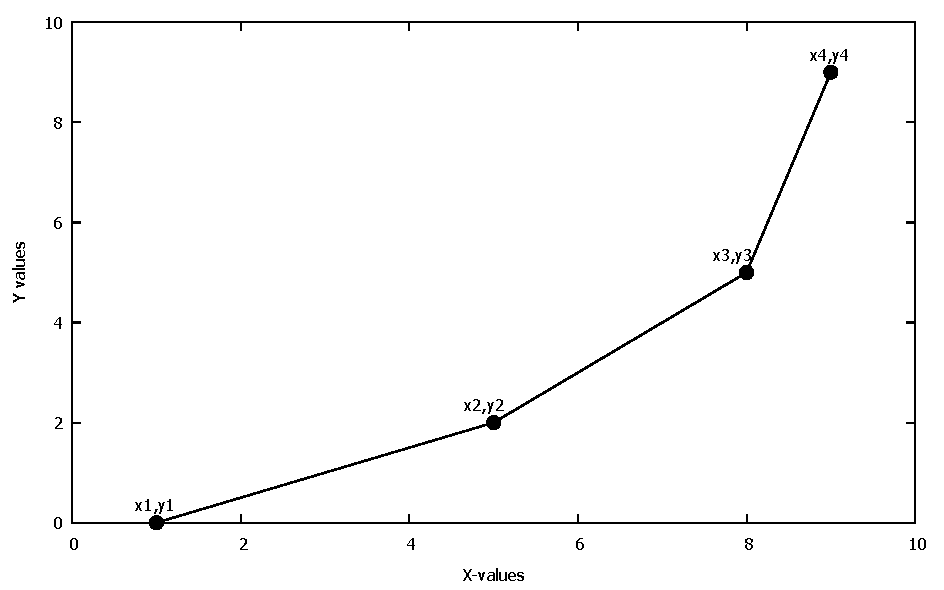
\includegraphics[width=12cm]{\FigDir/figure_AFGEN.pdf}
 \caption{Linear interpolation}
 \label{fig:afgen}    
\end{figure}

The array belonging to this example has to be filled as:\\

\begin{center}
\begin{tabular}{lcccccccc}
Place & (1)& (2)& (3)& (4)& (5)& (6)& (7)& (8)\\
Value & X$_{{\rm 1}}$ & Y$_{{\rm 1}}$   & X$_{{\rm 2}}$& Y$_{{\rm 2}}$   & X$_{{\rm 3}}$ & Y$_{{\rm 3}}$   & X$_{{\rm 4}}$ & Y$_{{\rm 4}}$\\
\end{tabular}
\end{center}

The arguments of the AFGEN function in order of their place in the argument list are: name
of the table, number of pairs, X value to be interpolated. The X-values have to be arranged
from low to high values and are not allowed to be interchanged. Every X-value has to
precede its connected Y-value.

Three situations for interpolation can occur:

\begin{enumerate}
\item The argument {\it x} at which interpolation should take place is less or equal to the first
    X-value in the array. The Y-value is set to the first Y-value in the array.
\item The argument {\it x\/} value at which interpolation should take place is between the first
    and the last X-value in the array. The Y-value can now be found via linear
    interpolation. First the X values left and right from the argument {\it x\/} have to be
    detected, then the Y-value can be calculated:\\
    \begin{equation*}
    y~=~ Y _{n-1} ~+~ (\, x\, -\, X _{n-1} \, )\,{\frac{ Y _{n} \, -\, Y _{n-1} }{X _{n} \, -\, X _{n-1} }}
    \end{equation*}
\item The argument {\it x\/} at which interpolation should take place is equal to or larger then the
    last X-value in the array. The Y-value is set to the last Y-value in the array.
\end{enumerate}